\pagestyle{empty}
\tikzstyle{every picture}+=[remember picture]
\everymath{\displaystyle}
\begin{figure}[!ht]

\hspace{0.5cm} Events history:
\([ \thinspace
\tikz\node [fill=red!20,draw,circle] (n1) {}; \thinspace
\tikz\node [fill=green!20,draw,circle] (n2){}; \thinspace
\tikz\node [fill=blue!20,draw,circle] (n3) {}; \thinspace
\tikz\node [fill=black!20,draw,circle] (n4){}; \thinspace
]
\vspace{1cm}
\)

\centering
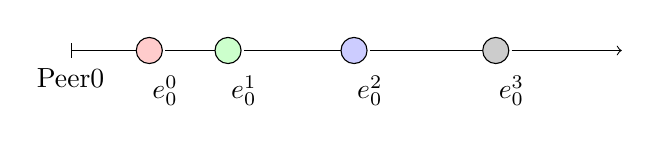
\begin{tikzpicture}
\draw[|-] (1,0) node[below=1mm]{Peer0} -- (2,0) node{\tikz[baseline]{
	\node[fill=red!20,draw,circle] (e0){};
}};
\draw[-] (2.2,0) node[below=2mm]{$e^0_0$} -- (3,0) node{\tikz[baseline]{
	\node[fill=green!20,draw,circle] (e1){};
}};
\draw[-] (3.2,0) node[below=2mm]{$e^1_0$} -- (4.6,0) node{\tikz[baseline]{
	\node[fill=blue!20,draw,circle] (e2){};
}};
\draw[-] (4.8,0) node[below=2mm]{$e^2_0$} -- (6.4,0) node{\tikz[baseline]{
	\node[fill=black!20,draw,circle] (e3){};
}};
\draw[->] (6.6,0) node[below=2mm]{$e^3_0$} -- (8,0) node[below=1mm]{};
\end{tikzpicture}

\begin{tikzpicture}[overlay]
        \path[->] (n1) edge [out=-90, in=120] (e0);
        \path[->] (n2) edge [out=-90, in=120] (e1);
        \path[->] (n3) edge [out=-70, in=135] (e2);
        \path[->] (n4) edge [out=-70, in=135] (e3);
\end{tikzpicture}

  \caption{The sequence of events stored in the peer array's  and scheduled in the time space diagram.}
\end{figure}
